 
%% bare_conf.tex
%% V1.3
%% 2007/01/11
%% by Michael Shell
%% See:
%% http://www.michaelshell.org/
%% for current contact information.
%%
%% This is a skeleton file demonstrating the use of IEEEtran.cls
%% (requires IEEEtran.cls version 1.7 or later) with an IEEE conference report.
%%
%% Support sites:
%% http://www.michaelshell.org/tex/ieeetran/
%% http://www.ctan.org/tex-archive/macros/latex/contrib/IEEEtran/
%% and
%% http://www.ieee.org/

%%*************************************************************************
%% Legal Notice:
%% This code is offered as-is without any warranty either expressed or
%% implied; without even the implied warranty of MERCHANTABILITY or
%% FITNESS FOR A PARTICULAR PURPOSE! 
%% User assumes all risk.
%% In no event shall IEEE or any contributor to this code be liable for
%% any damages or losses, including, but not limited to, incidental,
%% consequential, or any other damages, resulting from the use or misuse
%% of any information contained here.
%%
%% All comments are the opinions of their respective authors and are not
%% necessarily endorsed by the IEEE.
%%
%% This work is distributed under the LaTeX Project Public License (LPPL)
%% ( http://www.latex-project.org/ ) version 1.3, and may be freely used,
%% distributed and modified. A copy of the LPPL, version 1.3, is included
%% in the base LaTeX documentation of all distributions of LaTeX released
%% 2003/12/01 or later.
%% Retain all contribution notices and credits.
%% ** Modified files should be clearly indicated as such, including  **
%% ** renaming them and changing author support contact information. **
%%
%% File list of work: IEEEtran.cls, IEEEtran_HOWTO.pdf, bare_adv.tex,
%%                    bare_conf.tex, bare_jrnl.tex, bare_jrnl_compsoc.tex
%%*************************************************************************

% *** Authors should verify (and, if needed, correct) their LaTeX system  ***
% *** with the testflow diagnostic prior to trusting their LaTeX platform ***
% *** with production work. IEEE's font choices can trigger bugs that do  ***
% *** not appear when using other class files.                            ***
% The testflow support page is at:
% http://www.michaelshell.org/tex/testflow/



% Note that the a4report option is mainly intended so that authors in
% countries using A4 can easily print to A4 and see how their reports will
% look in print - the typesetting of the document will not typically be
% affected with changes in report size (but the bottom and side margins will).
% Use the testflow package mentioned above to verify correct handling of
% both report sizes by the user's LaTeX system.
%
% Also note that the "draftcls" or "draftclsnofoot", not "draft", option
% should be used if it is desired that the figures are to be displayed in
% draft mode.
%
\documentclass[9pt,conference]{IEEEtran}
\usepackage{amssymb}
% Add the compsoc option for Computer Society conferences.
%
% If IEEEtran.cls has not been installed into the LaTeX system files,
% manually specify the path to it like:
% \documentclass[conference]{../sty/IEEEtran}





% Some very useful LaTeX packages include:
% (uncomment the ones you want to load)


% *** MISC UTILITY PACKAGES ***
%
%\usepackage{ifpdf}
% Heiko Oberdiek's ifpdf.sty is very useful if you need conditional
% compilation based on whether the output is pdf or dvi.
% usage:
% \ifpdf
%   % pdf code
% \else
%   % dvi code
% \fi
% The latest version of ifpdf.sty can be obtained from:
% http://www.ctan.org/tex-archive/macros/latex/contrib/oberdiek/
% Also, note that IEEEtran.cls V1.7 and later provides a builtin
% \ifCLASSINFOpdf conditional that works the same way.
% When switching from latex to pdflatex and vice-versa, the compiler may
% have to be run twice to clear warning/error messages.





% *** CITATION PACKAGES ***
%
%\usepackage{cite}
% cite.sty was written by Donald Arseneau
% V1.6 and later of IEEEtran pre-defines the format of the cite.sty package
%  \cite{} output to follow that of IEEE. Loading the cite package will
% result in citation numbers being automatically sorted and properly
% "compressed/ranged". e.g., [1], [9], [2], [7], [5], [6] without using
% cite.sty will become [1], [2], [5]--[7], [9] using cite.sty. cite.sty's
%  \cite will automatically add leading space, if needed. Use cite.sty's
% noadjust option (cite.sty V3.8 and later) if you want to turn this off.
% cite.sty is already installed on most LaTeX systems. Be sure and use
% version 4.0 (2003-05-27) and later if using hyperref.sty. cite.sty does
% not currently provide for hyperlinked citations.
% The latest version can be obtained at:
% http://www.ctan.org/tex-archive/macros/latex/contrib/cite/
% The documentation is contained in the cite.sty file itself.






% *** GRAPHICS RELATED PACKAGES ***
%
\ifCLASSINFOpdf
  \usepackage[pdftex]{graphicx}
  % declare the path(s) where your graphic files are
  % \graphicspath{{../pdf/}{../jpeg/}}
  % and their extensions so you won't have to specify these with
  % every instance of \includegraphics
  % \DeclareGraphicsExtensions{.pdf,.jpeg,.png}
\else
  % or other class option (dvipsone, dvipdf, if not using dvips). graphicx
  % will default to the driver specified in the system graphics.cfg if no
  % driver is specified.
  % \usepackage[dvips]{graphicx}
  % declare the path(s) where your graphic files are
  % \graphicspath{{../eps/}}
  % and their extensions so you won't have to specify these with
  % every instance of \includegraphics
  % \DeclareGraphicsExtensions{.eps}
\fi
% graphicx was written by David Carlisle and Sebastian Rahtz. It is
% required if you want graphics, photos, etc. graphicx.sty is already
% installed on most LaTeX systems. The latest version and documentation can
% be obtained at: 
% http://www.ctan.org/tex-archive/macros/latex/required/graphics/
% Another good source of documentation is "Using Imported Graphics in
% LaTeX2e" by Keith Reckdahl which can be found as epslatex.ps or
% epslatex.pdf at: http://www.ctan.org/tex-archive/info/
%
% latex, and pdflatex in dvi mode, support graphics in encapsulated
% postscript (.eps) format. pdflatex in pdf mode supports graphics
% in .pdf, .jpeg, .png and .mps (metapost) formats. Users should ensure
% that all non-photo figures use a vector format (.eps, .pdf, .mps) and
% not a bitmapped formats (.jpeg, .png). IEEE frowns on bitmapped formats
% which can result in "jaggedy"/blurry rendering of lines and letters as
% well as large increases in file sizes.
%
% You can find documentation about the pdfTeX application at:
% http://www.tug.org/applications/pdftex





% *** MATH PACKAGES ***
%
%\usepackage[cmex10]{amsmath}
% A popular package from the American Mathematical Society that provides
% many useful and powerful commands for dealing with mathematics. If using
% it, be sure to load this package with the cmex10 option to ensure that
% only type 1 fonts will utilized at all point sizes. Without this option,
% it is possible that some math symbols, particularly those within
% footnotes, will be rendered in bitmap form which will result in a
% document that can not be IEEE Xplore compliant!
%
% Also, note that the amsmath package sets \interdisplaylinepenalty to 10000
% thus preventing page breaks from occurring within multiline equations. Use:
%\interdisplaylinepenalty=2500
% after loading amsmath to restore such page breaks as IEEEtran.cls normally
% does. amsmath.sty is already installed on most LaTeX systems. The latest
% version and documentation can be obtained at:
% http://www.ctan.org/tex-archive/macros/latex/required/amslatex/math/





% *** SPECIALIZED LIST PACKAGES ***
%
\usepackage{algorithm}
\usepackage{algorithmic}
% algorithmic.sty was written by Peter Williams and Rogerio Brito.
% This package provides an algorithmic environment fo describing algorithms.
% You can use the algorithmic environment in-text or within a figure
% environment to provide for a floating algorithm. Do NOT use the algorithm
% floating environment provided by algorithm.sty (by the same authors) or
% algorithm2e.sty (by Christophe Fiorio) as IEEE does not use dedicated
% algorithm float types and packages that provide these will not provide
% correct IEEE style captions. The latest version and documentation of
% algorithmic.sty can be obtained at:
% http://www.ctan.org/tex-archive/macros/latex/contrib/algorithms/
% There is also a support site at:
% http://algorithms.berlios.de/index.html
% Also of interest may be the (relatively newer and more customizable)
% algorithmicx.sty package by Szasz Janos:
% http://www.ctan.org/tex-archive/macros/latex/contrib/algorithmicx/




% *** ALIGNMENT PACKAGES ***
%
%\usepackage{array}
% Frank Mittelbach's and David Carlisle's array.sty patches and improves
% the standard LaTeX2e array and tabular environments to provide better
% appearance and additional user controls. As the default LaTeX2e table
% generation code is lacking to the point of almost being broken with
% respect to the quality of the end results, all users are strongly
% advised to use an enhanced (at the very least that provided by array.sty)
% set of table tools. array.sty is already installed on most systems. The
% latest version and documentation can be obtained at:
% http://www.ctan.org/tex-archive/macros/latex/required/tools/


%\usepackage{mdwmath}
%\usepackage{mdwtab}
% Also highly recommended is Mark Wooding's extremely powerful MDW tools,
% especially mdwmath.sty and mdwtab.sty which are used to format equations
% and tables, respectively. The MDWtools set is already installed on most
% LaTeX systems. The lastest version and documentation is available at:
% http://www.ctan.org/tex-archive/macros/latex/contrib/mdwtools/


% IEEEtran contains the IEEEeqnarray family of commands that can be used to
% generate multiline equations as well as matrices, tables, etc., of high
% quality.


%\usepackage{eqparbox}
% Also of notable interest is Scott Pakin's eqparbox package for creating
% (automatically sized) equal width boxes - aka "natural width parboxes".
% Available at:
% http://www.ctan.org/tex-archive/macros/latex/contrib/eqparbox/





% *** SUBFIGURE PACKAGES ***
%\usepackage[tight,footnotesize]{subfigure}
% subfigure.sty was written by Steven Douglas Cochran. This package makes it
% easy to put subfigures in your figures. e.g., "Figure 1a and 1b". For IEEE
% work, it is a good idea to load it with the tight package option to reduce
% the amount of white space around the subfigures. subfigure.sty is already
% installed on most LaTeX systems. The latest version and documentation can
% be obtained at:
% http://www.ctan.org/tex-archive/obsolete/macros/latex/contrib/subfigure/
% subfigure.sty has been superceeded by subfig.sty.



%\usepackage[caption=false]{caption}
%\usepackage[font=footnotesize]{subfig}
% subfig.sty, also written by Steven Douglas Cochran, is the modern
% replacement for subfigure.sty. However, subfig.sty requires and
% automatically loads Axel Sommerfeldt's caption.sty which will override
% IEEEtran.cls handling of captions and this will result in nonIEEE style
% figure/table captions. To prevent this problem, be sure and preload
% caption.sty with its "caption=false" package option. This is will preserve
% IEEEtran.cls handing of captions. Version 1.3 (2005/06/28) and later 
% (recommended due to many improvements over 1.2) of subfig.sty supports
% the caption=false option directly:
%\usepackage[caption=false,font=footnotesize]{subfig}
%
% The latest version and documentation can be obtained at:
% http://www.ctan.org/tex-archive/macros/latex/contrib/subfig/
% The latest version and documentation of caption.sty can be obtained at:
% http://www.ctan.org/tex-archive/macros/latex/contrib/caption/




% *** FLOAT PACKAGES ***
%
%\usepackage{fixltx2e}
% fixltx2e, the successor to the earlier fix2col.sty, was written by
% Frank Mittelbach and David Carlisle. This package corrects a few problems
% in the LaTeX2e kernel, the most notable of which is that in current
% LaTeX2e releases, the ordering of single and double column floats is not
% guaranteed to be preserved. Thus, an unpatched LaTeX2e can allow a
% single column figure to be placed prior to an earlier double column
% figure. The latest version and documentation can be found at:
% http://www.ctan.org/tex-archive/macros/latex/base/



%\usepackage{stfloats}
% stfloats.sty was written by Sigitas Tolusis. This package gives LaTeX2e
% the ability to do double column floats at the bottom of the page as well
% as the top. (e.g., "\begin{figure*}[!b]" is not normally possible in
% LaTeX2e). It also provides a command:
%\fnbelowfloat
% to enable the placement of footnotes below bottom floats (the standard
% LaTeX2e kernel puts them above bottom floats). This is an invasive package
% which rewrites many portions of the LaTeX2e float routines. It may not work
% with other packages that modify the LaTeX2e float routines. The latest
% version and documentation can be obtained at:
% http://www.ctan.org/tex-archive/macros/latex/contrib/sttools/
% Documentation is contained in the stfloats.sty comments as well as in the
% presfull.pdf file. Do not use the stfloats baselinefloat ability as IEEE
% does not allow \baselineskip to stretch. Authors submitting work to the
% IEEE should note that IEEE rarely uses double column equations and
% that authors should try to avoid such use. Do not be tempted to use the
% cuted.sty or midfloat.sty packages (also by Sigitas Tolusis) as IEEE does
% not format its reports in such ways.





% *** PDF, URL AND HYPERLINK PACKAGES ***
%
\usepackage{url}
% url.sty was written by Donald Arseneau. It provides better support for
% handling and breaking URLs. url.sty is already installed on most LaTeX
% systems. The latest version can be obtained at:
% http://www.ctan.org/tex-archive/macros/latex/contrib/misc/
% Read the url.sty source comments for usage information. Basically,
% \url{my_url_here}.





% *** Do not adjust lengths that control margins, column widths, etc. ***
% *** Do not use packages that alter fonts (such as pslatex).         ***
% There should be no need to do such things with IEEEtran.cls V1.6 and later.
% (Unless specifically asked to do so by the journal or conference you plan
% to submit to, of course. )


% correct bad hyphenation here
\hyphenation{op-tical net-works semi-conduc-tor}


\begin{document}

% report title
% can use linebreaks \\ within to get better formatting as desired

\title{Enhancing the Thymio to perform Search and Exploration} 

\author{
    Simone Eandi \\
    eandis@usi.ch
	\and
	Marco Ferri \\
	ferrima@usi.ch
	\and 
	Nadia Younis \\
	younin@usi.ch
}

\maketitle

% conference reports do not typically use \thanks and this command
% is locked out in conference mode. If really needed, such as for
% the acknowledgment of grants, issue a \IEEEoverridecommandlockouts
% after \documentclass

% for over three affiliations, or if they all won't fit within the width
% of the page, use this alternative format:
% 
%\author{\IEEEauthorblockN{Michael Shell\IEEEauthorrefmark{1},
%Homer Simpson\IEEEauthorrefmark{2},
%James Kirk\IEEEauthorrefmark{3}, 
%Montgomery Scott\IEEEauthorrefmark{3} and
%Eldon Tyrell\IEEEauthorrefmark{4}}
%\IEEEauthorblockA{\IEEEauthorrefmark{1}School of Electrical and Computer Engineering\\
%Georgia Institute of Technology,
%Atlanta, Georgia 30332--0250\\ Email: see http://www.michaelshell.org/contact.html}
%\IEEEauthorblockA{\IEEEauthorrefmark{2}Twentieth Century Fox, Springfield, USA\\
%Email: homer@thesimpsons.com}
%\IEEEauthorblockA{\IEEEauthorrefmark{3}Starfleet Academy, San Francisco, California 96678-2391\\
%Telephone: (800) 555--1212, Fax: (888) 555--1212}
%\IEEEauthorblockA{\IEEEauthorrefmark{4}Tyrell Inc., 123 Replicant Street, Los Angeles, California 90210--4321}}




% use for special report notices
%\IEEEspecialreportnotice{(Invited report)}




% make the title area
\maketitle


\begin{abstract}
%\boldmath
The object of this project was to extend the capabilities of the Thmyio robot to make it able to explore an unknown indoor environment while searching for a target, under the assumption that an external perfectly accurate localization was given. This was achieved by adding a LIDAR to the robot in order to greatly improve its ability to perceive the environment and implementing a set of ROS nodes to process its readings. A mapping routine was implemented to generate a 3D map of the environment from the point clouds produced by the LIDAR, detect obstacles and create a 2D occupancy grid of the traversable terrain. A template matching algorithm was also designed to detect the presence of a given target from its 3D model and the point cloud mapping of the environment. Then, a set of path planning routines were implemented that make use of the occupancy grid and the target detection module to compute the robot control inputs that allow it to perform map coverage and target reaching. Finally, a Gazebo model of the robot has been created and used to simulate the execution in several different indoor environments where very good results were observed both for the mapping and path planning tasks.
\end{abstract}

% IEEEtran.cls defaults to using nonbold math in the Abstract.
% This preserves the distinction between vectors and scalars. However,
% if the conference you are submitting to favors bold math in the abstract,
% then you can use LaTeX's standard command \boldmath at the very start
% of the abstract to achieve this. Many IEEE journals/conferences frown on
% math in the abstract anyway.


% no keywords


% For peer review reports, you can put extra information on the cover
% page as needed:
% \ifCLASSOPTIONpeerreview
% \begin{center} \bfseries EDICS Category: 3-BBND \end{center}
% \fi
%
% For peerreview reports, this IEEEtran command inserts a page break and
% creates the second title. It will be ignored for other modes.


\section{Introduction}

The goal of this project was to enhance the capabilities of the very famous Thymio robot \cite{Thymio} in order to make it able to perform search and exploration tasks within indoor environments with flat terrain. The code produced during the development of our project is open source and available on GitHub \cite{project-repo}.

The Thymio is a differential drive robot equipped with proximity sensor to detect close obstacles, these sensors have been proven to be insufficient alone to provide enough information to the robot about its environment to make it able to reliably and efficiently explore it; for this reason we have designed an improved version of the Thymio, named Thymar, which adopts a Lidar in order to enhance the perception capabilities of the base robot. 
The Thymar robot has been implemented as a set of ROS nodes, with each one corresponding to its own ROS package for better modularity, and tested in a simulated environment where it was asked to explore the surroundings in search for a target, defined as a sphere of 15 cm of radius. In particular, the implementation of the Thymar as been subdivided among three ROS nodes as follows: the \emph{thymar\_description} node is entirely responsible for the simulation of the robot, the \emph{thymar\_lidar} node takes care of mapping the environment and detecting the target while the \emph{thymar} node is the main node responsible for controlling the Thymar robot. For handling the robot simulation and relative visualizations, Gazebo \cite{gazebo} and RViz \cite{rviz} are being used in combination.

In the following document we will firstly describe the model used for the simulation of the Thymar robot, then we will go over how the mapping of unknown areas is performed, the technique used for identifying the presence of a specific target and the path planning approach used to control the robot; finally, the simulation results will be presented and discussed. 


%-----------------------


\section{Simulating the Thymar}

In order to simulate the Thymar robot, a model in Gazebo (figure \ref{fig:thymar_model}) has been created by using the \emph{thymio\_description} ROS package \cite{thymio_description} to simulate the Thymio robot and employing the \emph{velodyne\_simulator} package \cite{velodyne_simulator} to simulate a Velodyne VLP-16 Puck Lidar \cite{VLP16}. In particular, given that the proximity sensors of the Thymio have a maximum range of 15 cm, the LIDAR simulator has been setup to have a range between 14 cm and 3 meters in order to be complementary with them, furthermore, due to the limitations encountered while running the Gazebo simulation on the available hardware, the number of lasers projected by the Lidar within each vertical plane has been set to 64 and the overall reading frequency has been set to 0.5 Hz. The simulation of the Thymar has been completely integrated with ROS by making it publish and subscribe to a set of ROS topics under a common namespace (i.e. \emph{/thymar}) that can be used as I/O by any other ROS node. In particular, the model exposes its odometry on the \emph{~/odom} topic and it continuously publishes the readings from the LIDAR in the form of point cloud messages on the \emph{~/velodyne\_points} topic; finally, the Thymar can be fully controlled by publishing on the \emph{~/cmd\_vel} topic its linear and angular velocities. An important mention deserves the odometry computation: given that the aim of the Thymar was to map the environment under the assumption that its localization is given, the source for the odometry has been set to the Gazebo simulator instead of the differential drive encoder of the Thymar to prevent any error drift and have a perfect localization.

\begin{figure}[h!]
    \centering
    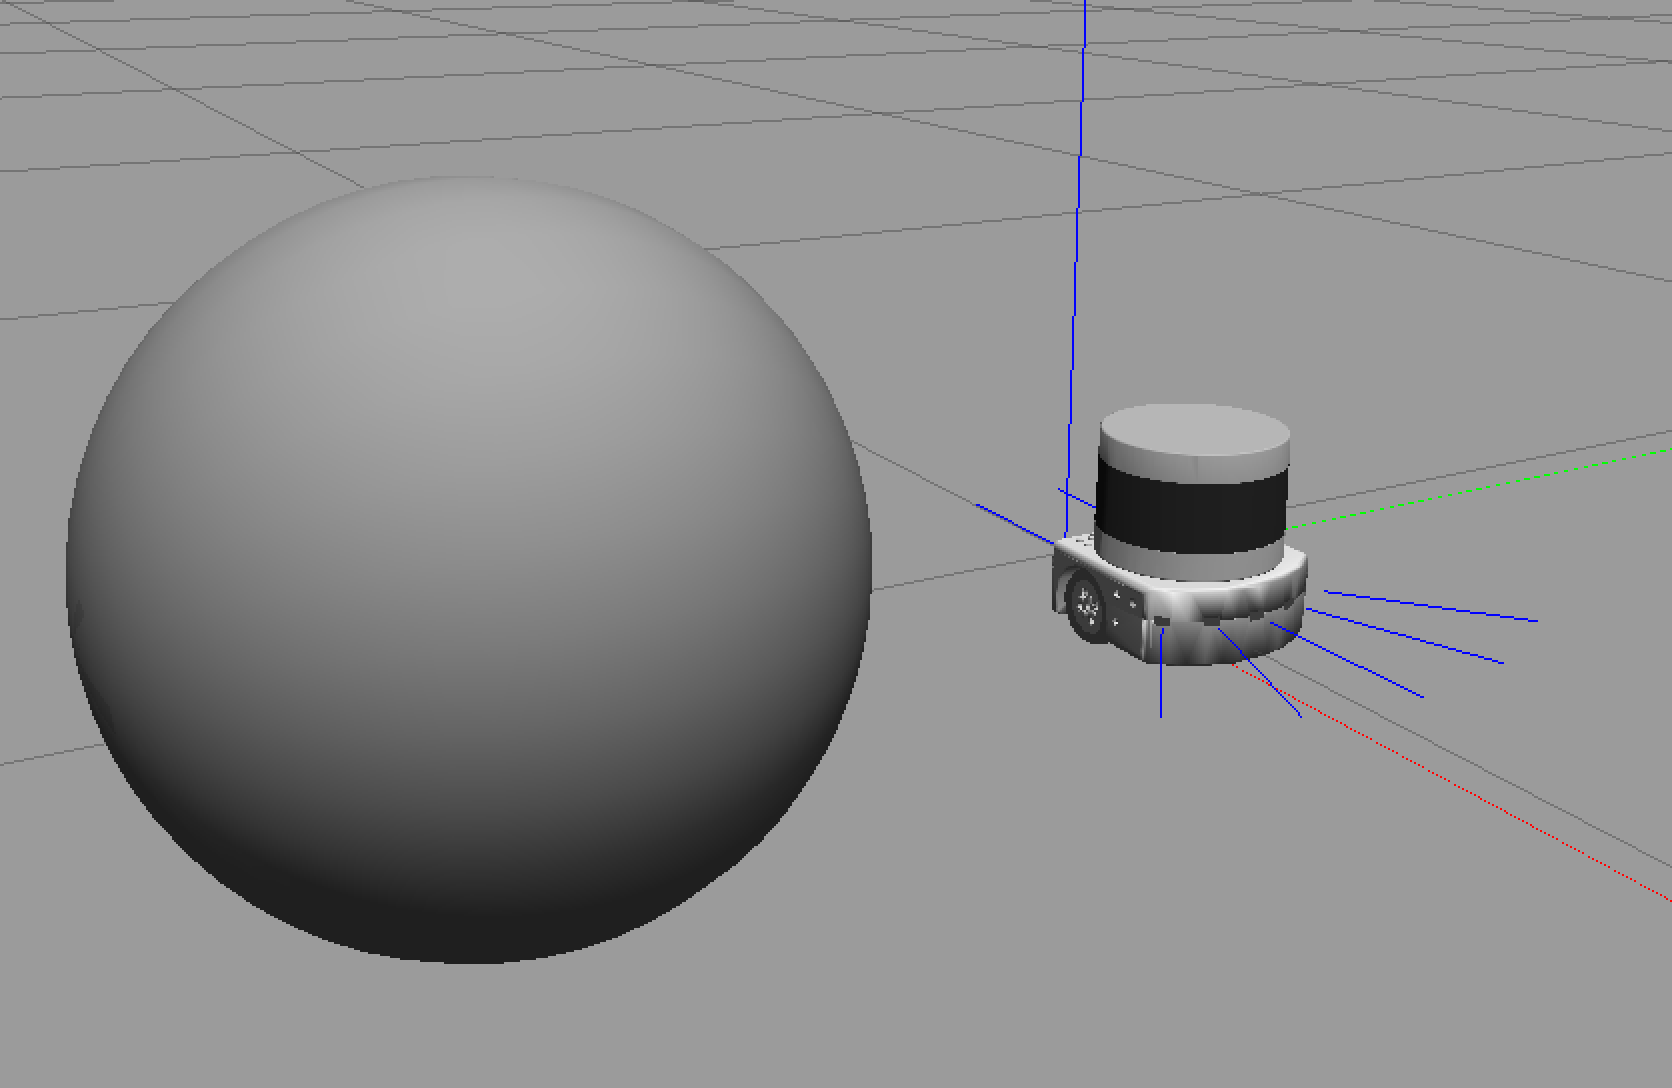
\includegraphics[width=1\linewidth]{images/01 robot.png}
    \caption{The Thymar robot and target model in Gazebo}
    \label{fig:thymar_model}
\end{figure}


%-----------------------


\section{Mapping}

All the computations related to the mapping of the environment have been assigned to the \emph{thymar\_lidar} node situated within the \emph{thymar\_lidar} package: it takes care of reading the point cloud messages from the simulation, combining them to create a 3-dimensional map of the environment, separating the obstacles from the traversable terrain and generating the 2D occupancy grid. The node has been implemented fully in C++ in order to make use of the PointCloudLibrary \cite{PCL} routines for handling point clouds and divided into an interface (Thymar\_lidar.cpp) that takes care of initializing the node and managing all the publications and subscriptions with ROS topics and a separate class (PointCloudMapper) which performs all the mapping computations related to point clouds.


\subsection{Mapping the environment}

Whenever a new point cloud message is published by the Thymar LIDAR, it is read and represented as a cloud of XYZ points PCL object exploiting the builtin automatic conversion between the ROS PointCloud2 type and the PCL types. Since the received point cloud is represented with respect to the Thymar reference frame, the pose of the robot at the moment of reading is retrieved from the \emph{~/odom} topic and used to apply a rigid transformation to the point cloud that brings it in the world reference frame defined as the frame associated to the odometry. Then, since the odometry are perfectly accurate, the 3D representation of the environment can be simply achieved by adding the new points to those currently in the world point cloud. In particular, to prevent the world point cloud to become extremely dense and computationally more expensive to analyse, downsampling is performed every time a new point cloud is added through a Voxel filter with leaf size of 5 cm in all directions (\textbf{algorithm \ref{alg_mapping}}). Remarkably, to avoid having to synchronize the odometry and point cloud messages, the point cloud produced by the LIDAR is read only when the Thymar velocity is purely linear, in which case no synchronization is necessary due to the low speed.

All the published topics can be visualized in RViz and figure \ref{fig:current-clouds} shows how different time steps LIDAR readings can be merged together for creating the 3D map of the environment by taking account the relative position with respect to the initial pose.

\begin{figure}[h!]
    \centering
    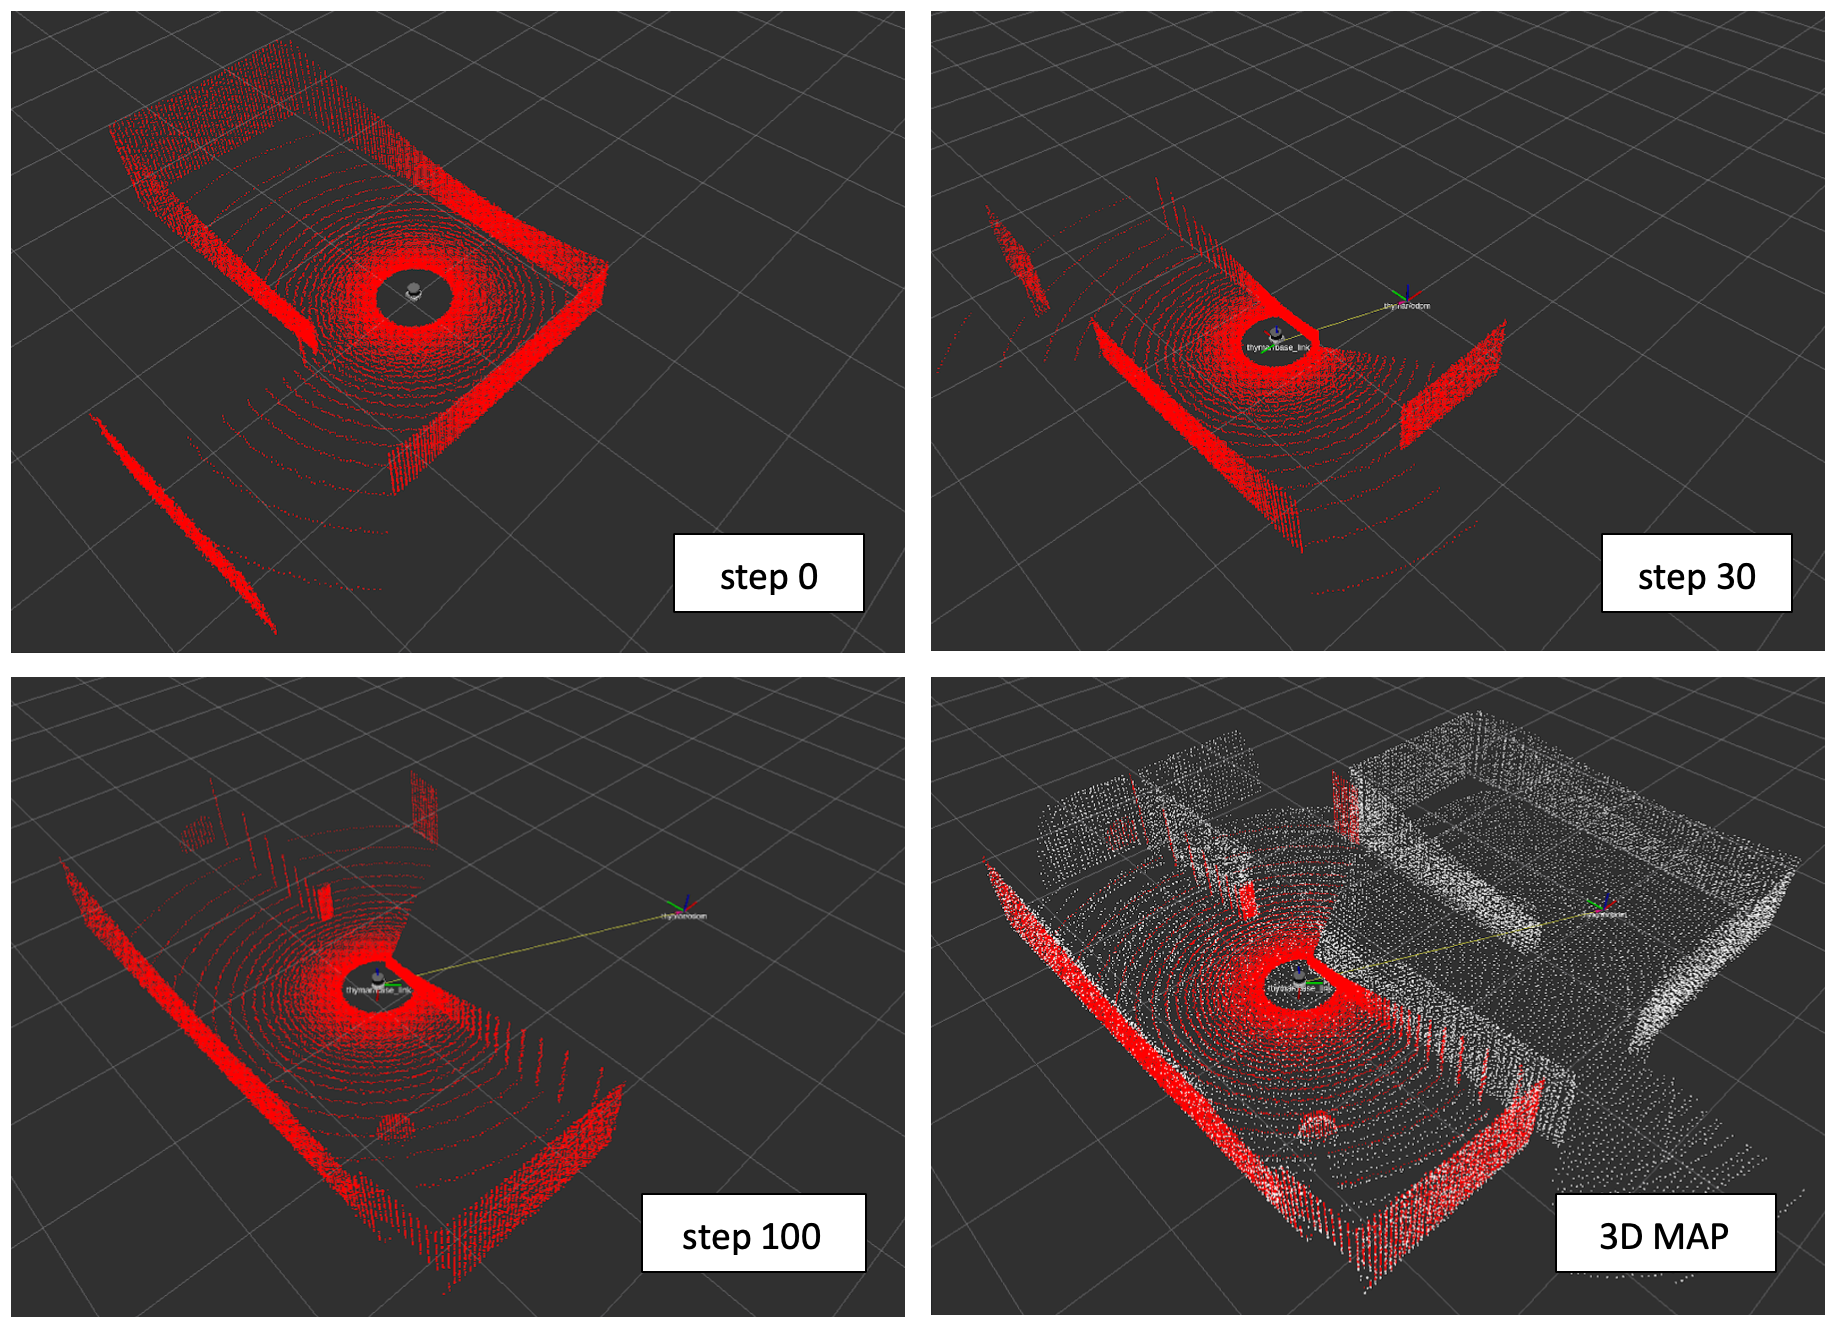
\includegraphics[width=1\linewidth]{images/03A merge.png}
    \caption{3D Map made up by merging point clouds at different time steps}
    \label{fig:current-clouds}
\end{figure}


\subsection{Separating obstacles and terrain}

The distinction between obstacles and terrain in the point cloud has been performed by simply applying a directional pass through filter which separates points according to their z coordinate with respect to a fixed threshold. Instead of performing this operation on the world point cloud, we chose to do it directly on each new point cloud after it is represented in the odometry reference frame, using an index-based approach to preserve the original cloud, and incrementally build the obstacles and terrain global point clouds in a similar fashion to what was done for the world cloud, including periodic downsampling (\textbf{algorithm \ref{alg_mapping}}). 


\subsection{Generating the occupancy grid}

In order to provide a simple and computationally efficient representation of the environment to be used for path planning, a 2D occupancy grid is generated from the point clouds. The grid has been defined as a matrix sufficiently large to cover all the environment where each cell represents the content of a 5cm by 5cm square region of the environment surface as a numeric value: a $-1$ value is assigned to unknown areas while a probability between $0$ and $100$ of being an obstacles is assigned to discovered areas (for simplicity a $0$ or $100$ binary approach has been used). The occupancy grid is built iteratively in a similar manner to what was done for the world point cloud by updating its content every time a new point cloud message is read. More in detail, the grid update is performed as follows: first, for each point in the new point cloud that has been found to belong to an obstacle, the corresponding cell in the occupancy grid is set to be an obstacle as well as all its neighboring cells to have a more robust representation, then all the points corresponding to terrain are parsed and the corresponding cells in the grid are set to traversable if and only if they were not previously labeled as terrain. Since each scan of the LIDAR acquires points belonging to the terrain arranged in a set of concentric rings, this result in a large groups of cells corresponding to points lying between those rings that remain undiscovered while obviously corresponding to terrain due to the LIDAR acquisition pattern; this issue is mitigated by post-processing the grid after each update in order to set to terrain all the unknown cells having a percentage of neighbors labeled as terrain above some threshold.

Figure \ref{fig:obstacles-2Dmap} shows how the point clouds corresponding to obstacles are used to generate the 2D map of known and unknown areas.

\begin{figure}[h!]
    \centering
    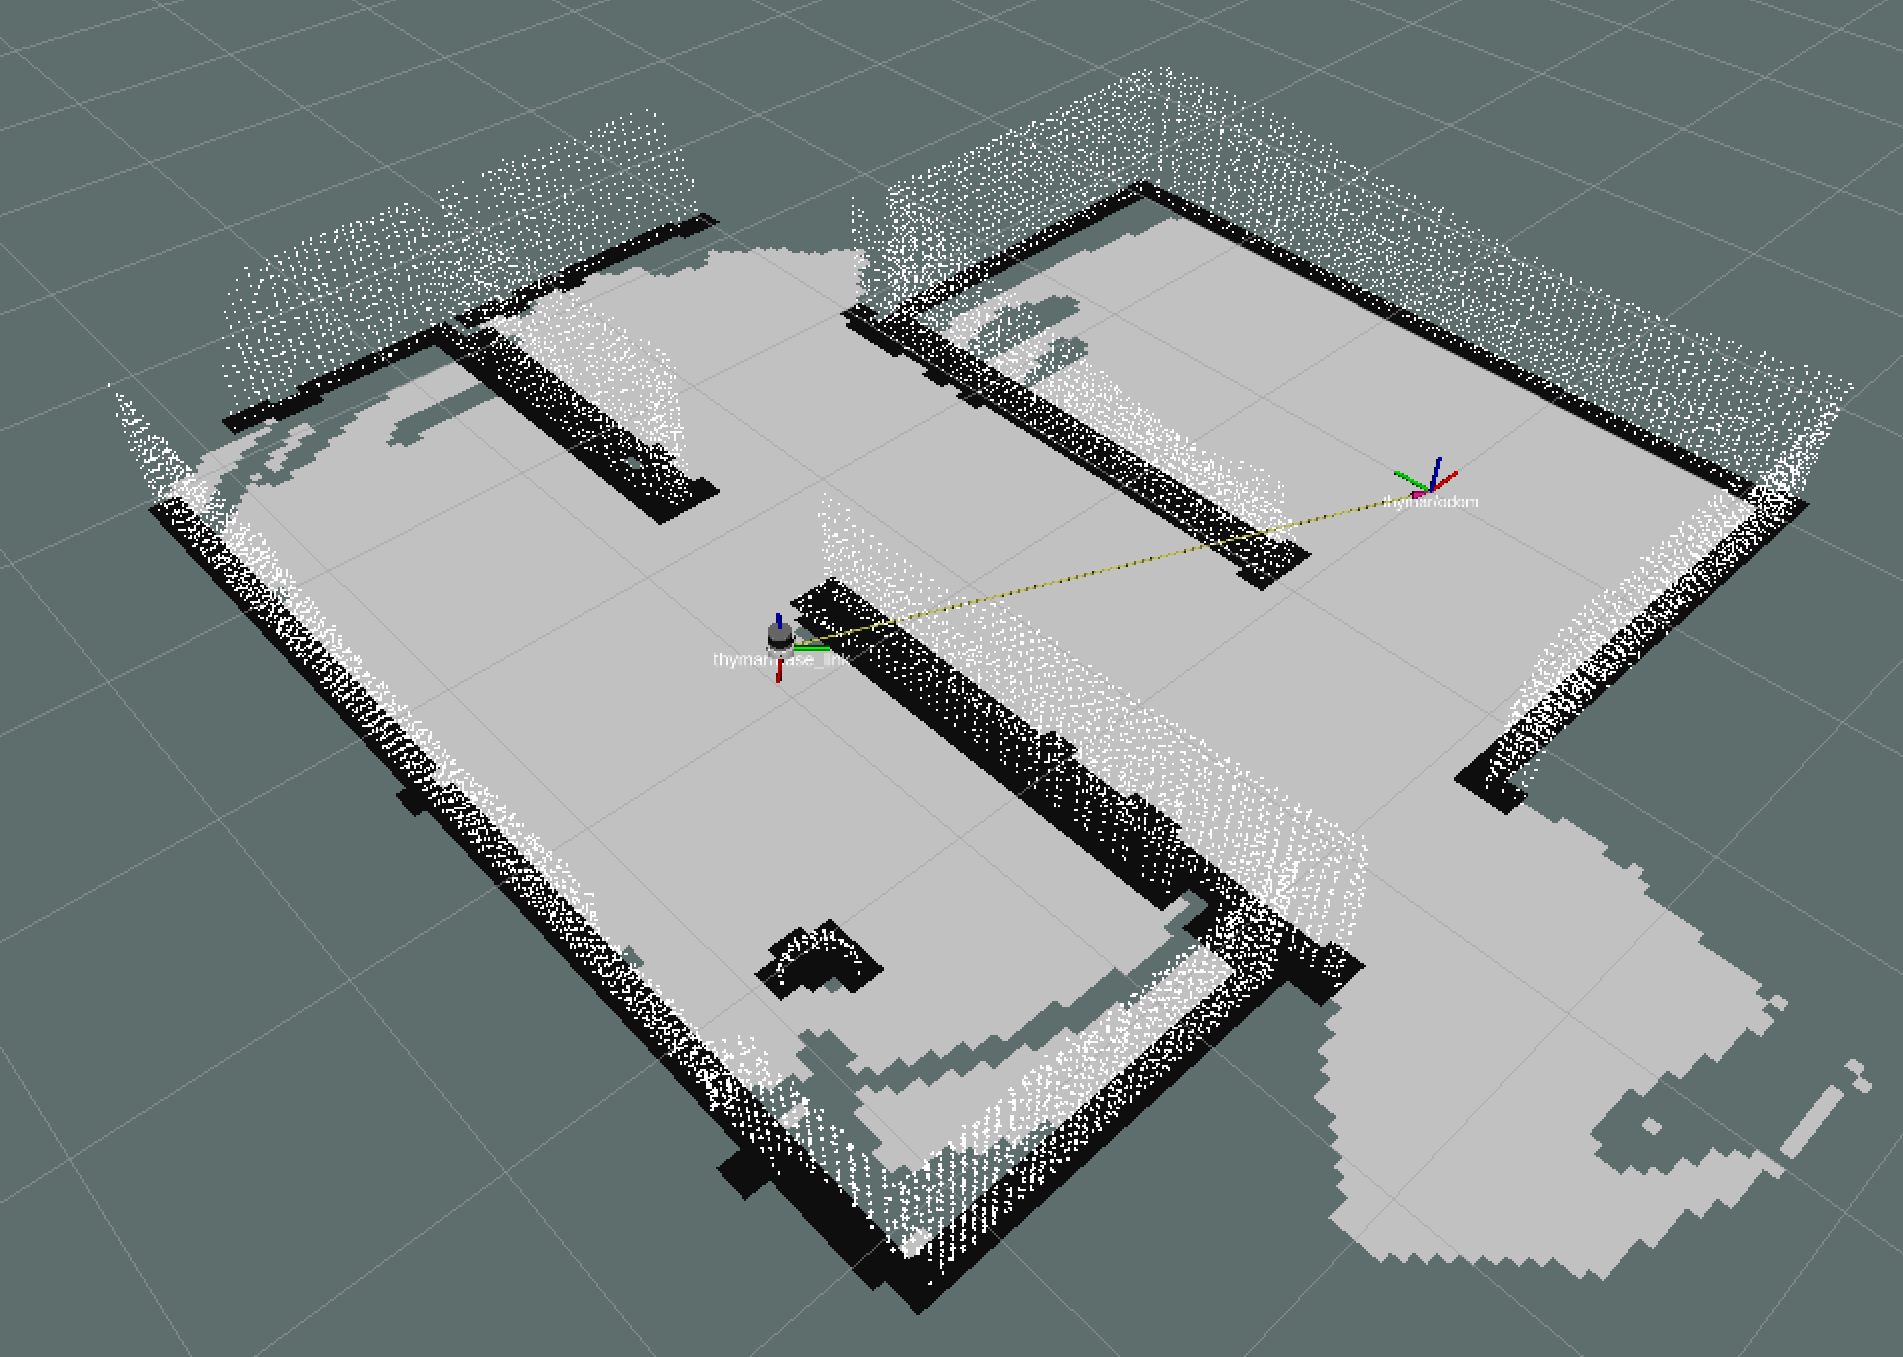
\includegraphics[width=1\linewidth]{images/02E obstacles+map2d crop.png}
    \caption{Obstacles point cloud and 2D map generated from it}
    \label{fig:obstacles-2Dmap}
\end{figure}

\begin{algorithm}[h!]
\caption{Mapping}
\label{alg_mapping}
\begin{algorithmic}
\STATE init publisher and subscriber
\STATE init word,obstacles and terrain point clouds
\STATE init occupancy grid
\WHILE{node running}
\IF{new point cloud message} 
\STATE represent the point cloud in the global frame
\STATE split point cloud into obstacles and terrain
\STATE add full point cloud to the world point cloud
\STATE add obstacles and terrain to the respective point clouds
\STATE downsample word obstacles and terrain clouds
\STATE update occupancy grid
\ENDIF
\STATE publish global point clouds and occupancy grid
\ENDWHILE 
\end{algorithmic}
\end{algorithm}


%-----------------------


\section{Target detection}

The \emph{thymar\_lidar} node is also responsible for detecting the given target, a sphere of 15cm of radius, whenever it is encountered during the exploration of the environment. The target detection is entirely performed by relying on the 3D point cloud generated by the LIDAR: given that the model of the target is assumed to be known, a template matching algorithm such as RANSAC can be exploited to detect the target. In particular, every time that a new point cloud is processed a clustering algorithm is applied on the global obstacle point cloud and only the clusters having a number of points within some threshold are selected, then, for each one of those, the RANSAC algorithm is applied: if for one of those cluster a fitting of the target model with a number of inliers above some threshold is obtained, then the target is considered to be found and the node publishes a marker in correspondence of the location of the fitted model (\textbf{algorithm \ref{code:target_detection}}). Notably, the detection routine is applied on the global obstacles point cloud and not on the individual readings, this was done because the target may actually not be recognizable until multiple point clouds from different views are joint together. Finally, note also that the filtering applied on the clusters of points have been made possible by the fact that the density of the point clouds is kept constant by the continuous downsampling operations and must be fine tuned on the specific model of the target.

\begin{algorithm}
\caption{Target detection}
\label{code:target_detection}
\begin{algorithmic}
\STATE init publisher and subscriber
\WHILE{node running}
\IF{new point cloud and target not found}
\STATE cluster the global obstacle point cloud
\STATE reject all clouds with a number of samples outside some range
\FOR{cluster in remaining clusters}
\STATE try to fit the target model in the cluster
\IF{fits}
\STATE set target to found
\STATE publish target location
\ENDIF
\ENDFOR
\ENDIF
\ENDWHILE 
\end{algorithmic}
\end{algorithm}


%-----------------------


\section{Basic exploration}
\label{sec:basic-exploration}

The exploration task is handled by the \textit{thymar} package, which is responsible for driving the Thymar in the selected world for mapping the environment in order to reach the target. This is achieved by defining a ROS controller that subscribes to the topics defined in the previous sections and uses them for computing how to move. Basically, the controller waits that the robot is ready (subscribers are working properly), for then handling the simulation through an infinite loop that evaluates the current situation and computes step-by-step robot's velocities.


\subsection{Sensing the environment}

From now on, the robot's perception about the environment will only consider the 2D map computed during the mapping phase, accordingly subscribing to the occupancy grid message published by the \textit{thymar\_lidar} node. Since this map is a grid discretization of the world with a specified resolution (5cm, in this case), the odometry information retrieved from the \textit{/odom} topic has to be properly converted into the corresponding occupancy grid cells in order to localize the robot within the map. Its position will be taken into account for evaluating what surrounds the robot at a certain moment. It is useful to remember that we use the Gazebo ground truth odometry for this task since we assume that localization is given correctly.


\subsection{Avoiding the obstacles}
\label{sec:obstacle-avoidance}

Given the map of the discovered environment and the robot position, a collision-avoidance policy can be defined for exploring the world without crashing into obstacles. Our basic exploration algorithm drives the robot straight forward since no obstacle is found, otherwise, the best turning direction is chosen for trying to follow a free way. Given the robot pose and orientation, obstacle detection is done by checking for free cells in the occupancy grid, considering the ones that are directly in front the robot within a chosen \textit{visibility} parameter (default 1 meter); for doing so, also robot width is taken into account during the computation.

Once an obstacle is found, an orientation searching phase starts. The algorithm firstly computes the best turning direction (left or right) by considering obstacles distances in the \texttt{90}-degrees cone in front of the robot, then a \textit{steering-step-degrees} parameter is used for evaluating possible orientations in that direction, using a doubled robot \textit{visibility} here. The search keeps going until a certain orientation leads to no obstacles in front of the robot or a substantial improvement is found in the distance between currently seen obstacles and the one that is obtained by turning in that orientation. If no way satisfies the condition, a try with decayed \textit{steering-step-degrees} is done and if the problem persists, then a random orientation between \texttt{-130} and \texttt{130} degrees is chosen.
Finally, the robot is guided by the controller for actually rotating until the chosen orientation is reached, so the obstacle avoidance algorithm restarts from the beginning.

This algorithm correctly works in most of the environments for exploring the available space until the target is reached, but easily leads to infinite loops in which the robot keeps traversing the same area over and over. Even if it does not happen, it is clear that this exploration technique is very inefficient for relatively large worlds. We will see in section \ref{sec:improve-exploration} how the problem has been taken out.


%-----------------------


\section{Reaching the target}
\label{sec:target-chasing}

While exploring, the target detection algorithm keeps running in parallel through the \textit{thymar\_lidar} node described before. As soon as the target is identified from the point cloud seen by the robot, its pose is published on a proper topic and a marker is published for better visualization in RViz. At this point, it is possible to retrieve both the robot and the target poses inside the map and this information can be used for driving the robot towards the target by using a path planning algorithm.


\subsection{Path planning}
\label{sec:path-planning}

Considering the available space as a grid, one of the most intuitive approaches for computing path planning is the A* algorithm \cite{wiki-A*}, which would treat the map cells as weighted graph nodes in order to find the least costing path between two nodes: the robot and the target. A* starts by visiting all the available cell that are reachable from the starting one (i.e., the robot pose) and then keeps iteratively exploring only the best ones accordingly to a given cost, which is computed by the exact number of (minimal) steps needed for reaching that cell plus the cost given by a heuristic function. As soon as the A* search finds the target cell, the best path for getting there is computed by back-propagating into the explored graph. In order to run A* on our problem, two parts of the algorithm must be defined: the heuristic and the neighborhood function. 

The heuristic function is used for evaluating the expected cost of reaching the goal from a certain node of the graph, without actually knowing the real cost the node will have at the end. This is used for choosing nodes from which the graph exploration should continue first, which according to the heuristic function will also be the ones nearest to the target node. In the examined case, this heuristic function can simply be the euclidean distance between the cell we are evaluating and the cell that corresponds to the target pose.

On the other side, the neighborhood function computes the neighbors of a given node in the graph, which means the cells that can be reached from that particular cell we are considering. In an obstacles-free 2D map the neighborhood function will return all the 8 adjacent cells of an input cell, but when dealing with obstacles some directions will be filtered out if they actually correspond to an obstacle. In practice, this is not enough for computing neighborhood in our problem, since the robot is not a single point but instead has s dimension which occupies more than one cell in the map. That is why a parameter is needed for considering how far the robot has to stay away from obstacles, that we will call \textit{safe-distance}; this value has to be compliant with robot width and also allow the robot itself to traverse passages that are wide enough for it to pass through. In real-world applications, this \textit{safe-distance} also has to consider possible noise in the localization task or eventually moving obstacles - which is not the case in our simulation.


\subsection{Path following}
\label{sec:path-following}

Once A* has found the target pose during the graph discovering (which represents the map), the path to reach that cell is reconstructed and finally published as a topic for visualization, as shown in figure \ref{fig:path-planning}. This path is then followed pose-by pose by the robot in order to reach the target pose. However, the path has the same grid resolution, so it contains all the cells that connect the robot and the goal which are 5cm wide each. Approaching poses which only differ by 5 centimeters is not easy nor worth it for the robot considering its size, so a defined number of poses are skipped in each step while following the path.

Given a single pose which the path is composed of, the robot uses a standard motion controller for reaching it. As a constraint, we limited the robot to just going straight or rotating, but not both moving forward and steering at the same time. Given the current pose and the goal, the robot initially turns around to face the pose to reach, then proceeds straight ahead until its coordinates in the world are relatively close to the goal pose. If a final orientation is set, the robot rotates again in order to satisfy the requirements.

\begin{figure}[h!]
    \centering
    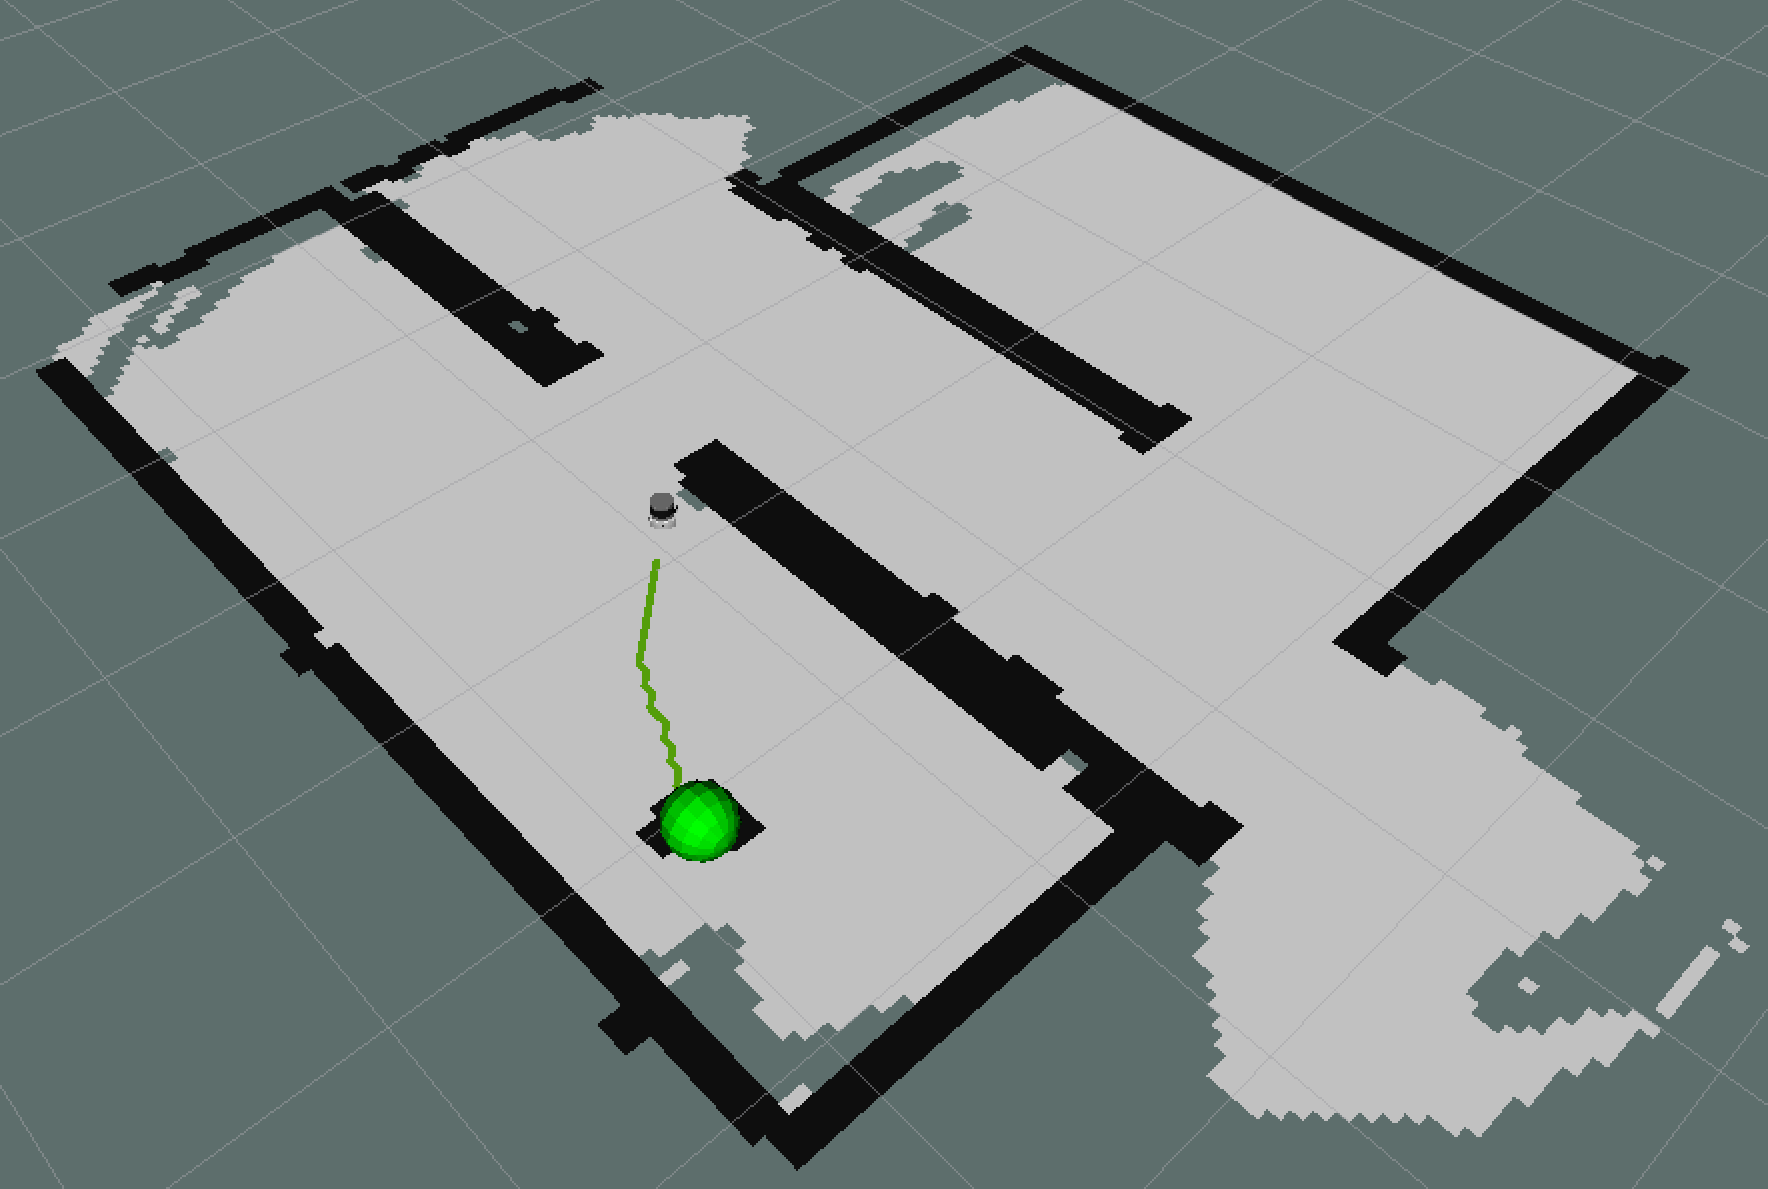
\includegraphics[width=1\linewidth]{images/02G target_plan crop.png}
    \caption{Path for reaching the target object}
    \label{fig:path-planning}
\end{figure}

\subsection{Back to the base}
\label{sec:back-to-base}

The path planning and tracking algorithms described in this section can actually be used to reach any point in the map as far as its coordinates are known. A common functionality after the target has been reached is to go back to a base (e.g., for returning what has been found). This goal is very simple to achieve by using what we have defined before since it is possible to set the initial pose of the robot as input for the path planning function for easily going back to the position where the robot has been spawned.


%-----------------------


\section{Improving the exploration}
\label{sec:improve-exploration}

The basic exploration approach defined in section \ref{sec:improve-exploration} resulted to be very inefficient and not useful at all in certain cases. That is why also the exploration phase has been redesigned using path planning.


\subsection{Exploring unknown areas}
\label{sec:unknown-exploration}

In order to optimize the exploration of the whole environment, it is useful to prioritize the reaching of those parts of the map which are marked as unknown in the occupancy grid. It is reasonable that always trying to explore unknown areas will certainly lead to also actually explore all the available space, and so, to the target. For achieving this, a searching approach is required and Dijkstra's algorithm \cite{wiki-dijkstra} has been chosen. It is a generalization of A* in which the weight of each node only accounts for the exact cost computed by the effort required for reaching that specific node from the starting point, without the usage of any heuristic function that points towards a final target node. 

Since the only difference with A* is the absence of the heuristic function, Dijkstra practically explores neighbor nodes in every direction such as a classic BFS algorithm \cite{wiki-bfs} would do. Another fundamental difference that has to be defined for our goal is when to stop the search. If when trying to reach a target the algorithm stops when the target is found in the searching graph, this time the stopping criteria is the discovery of an unknown area. If Dijkstra is stopped as soon as an unknown-marked cell is found, then the computed path would be the shortest way for reaching a currently unknown area, which will hopefully lead to the target object in the minimum time.

The computational resources required for computing Dijkstra are greater than A* since no preferred direction is chosen. Our algorithm always points to the nearest unknown cell but, while exploring, this cell will surely become known when approaching. That is why Dijkstra needs to be periodically recomputed in order to update the path the robot has to follow. A trade-off between exploration optimality and computational effort must be found and several experiments led to set the re-computation frequency every time the robot has approximately moved for 0.75 meters.

However, it sometimes happens that while moving the robot discovers new obstacles that lie on the path it is following (e.g., when approaching the corner of a wall). In this case, as soon as those obstacles are facing the robot an early path re-computation is required to avoid crashing against them.


\subsection{Map coverage}
\label{sec:coverage-exploration}

The interesting fact behind using Dijkstra for reaching unknown areas is that the same approach can be actually used for handling a map coverage task, so the mapping of all available traversable terrain. This is particularly useful when a robot is placed in an unknown environment and has to map it, which can have several purposes in real-world applications.

The algorithm used for exploration is exactly the same for map coverage and the only difference relies on failures management. While searching for the target, if Dijkstra is not able to find unknown areas and the target has not been found yet, then it would mean that (assuming there is no error in the mapping task) the target is not present in the environment. However, it can be also stated that the entire environment has been explored. Similarly, if the current objective is to discover the whole map instead of finding the target, a failure in the Dijkstra algorithm means the task has been successfully achieved.

It also has to be noticed that achieving map coverage is actually even more expensive than just exploring the map since the unknown areas could now be very far from the current position, especially if during the exploration some small parts of the environment have been left out. In order to avoid frequent and very long path updates, a workaround has been taken into consideration: if the path is longer than 5 meters, then the re-computation happens just when at least half of it has been traveled.


\subsection{State machine}

Given all the features discussed until now, the practical possibilities with such a robot are very powerful. For controlling the robot goals step by step, some states and relative transitions have been defined.

\begin{itemize}
    \item \texttt{exploring\_random}: tells the robot to follow the obstacle avoidance policy defined in section \ref{sec:obstacle-avoidance}
    \item \texttt{exploring\_smart}: tells the robot to prioritize the exploration of closest unknown areas such as described in section \ref{sec:unknown-exploration}
    \item \texttt{exploring\_coverage}: tells the robot to achieve map coverage as seen in section \ref{sec:coverage-exploration}
    \item \texttt{chasing\_target}: tells the robot to do path planning in order to reach the target as described in section \ref{sec:path-planning}
    \item \texttt{chasing\_goal}: utility state that is used in combination with other tasks for reaching a given pose in the map, such as simply avoiding an obstacle or following the path with the algorithm briefly discussed in the path following section \ref{sec:path-following}
    \item \texttt{returning}: tells the robot to enable path planning towards the initial pose as we have seen in section \ref{sec:back-to-base}
    \item \texttt{end}: final state, used for terminating the program
\end{itemize}

A combination of all these states can be easily defined for solving different types of problems. An exhaustive simulation will be made by setting the robot for finding the target, reaching it, explore all the maps and the finally return to the base. However, other combinations can be defined such as, for example, the possibility of returning as soon as the target has been found or simply achieving map coverage without anything else.


%-----------------------


\section{Conclusion}

Some basic techniques for driving a wheeled robot in search of a target object have been presented. Using a LIDAR for sensing the unknown environment, a 2D map has been created for then applying two different types of path planning for finding a given target and exploring all the available space. Working with the point clouds for defining the map works very well, so it does path planning on the resulting map. Several environments with different characteristics have been tested out and results are very promising. It is cool to notice that our A* implementation also works properly when the target pose is known, but actually resides inside an unknown area; in this case, paths updates are very frequent and the map is created while approaching the target, as shown in figure \ref{fig:target-in-unknown-area} and video \cite{demo-unknown-target-reaching}.

However, for taking our robot into the real-world some other implementations would be needed, later discussed in section \ref{sec:future-works}.

\begin{figure}[h!]
    \centering
    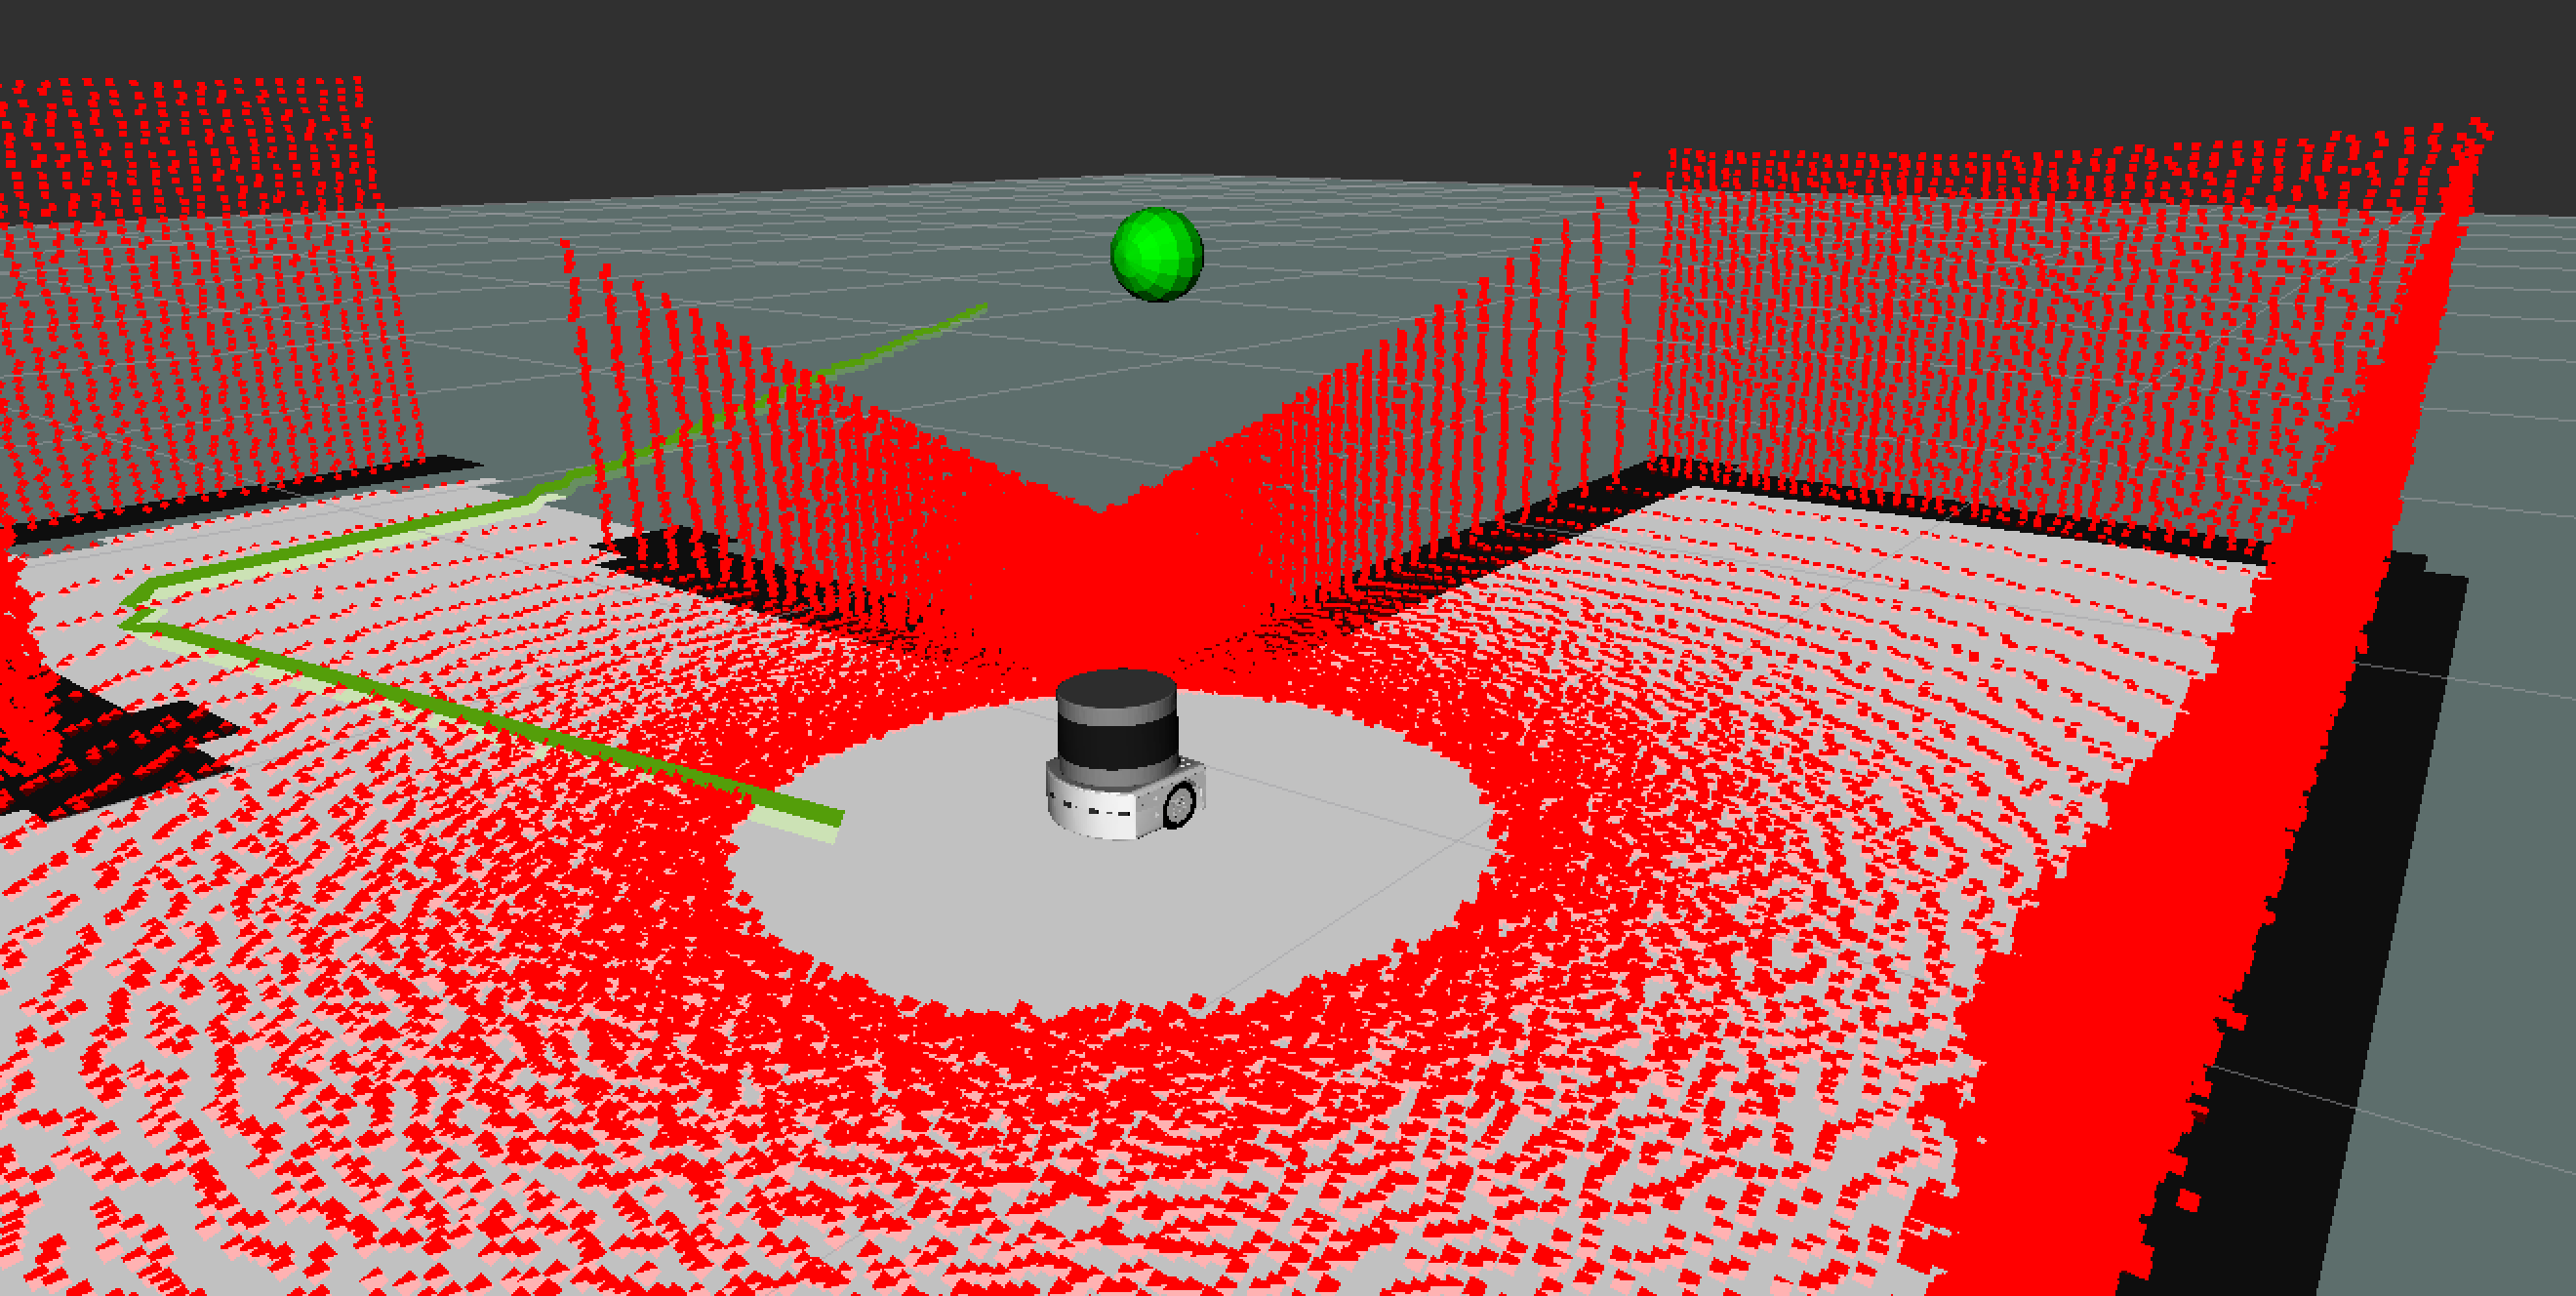
\includegraphics[width=1\linewidth]{images/presentation-cover.png}
    \caption{Path plan for reaching a target placed in unknown area}
    \label{fig:target-in-unknown-area}
\end{figure}


\subsection{Demos}

Some videos \cite{demo-videos} showing Gazebo + RViz simulations are available together with an interactive presentation \cite{demo-presentation} which summarizes what has been done. 


\subsection{Future works}
\label{sec:future-works}

Bringing the robot to the real-world requires further tasks:

\begin{itemize}
    \item Target recognition could be improved for better detecting target also when obstacles that are similar to the target in shape and size are available in the environment (e.g., cylinders with the same radius of our target sphere)
    \item During development, we assumed that odometry is given and correct for simplifying the environment we work with (we use the information that Gazebo provides us); actually, real-world implementations require both the Mapping and Localization tasks to be solved with proper SLAM techniques, also because the odometry information retrieved by the built-in robot sensors are too noisy for being considered acceptable for the mapping task, as shown in one available video \cite{demo-error-odom}
    \item A reasonable alternative for reducing noise in the mapping task is to also implement an Iterative Closest Point algorithm \cite{wiki-icp}
\end{itemize}


%----------------------------------------------


{\small
	\bibliographystyle{ieee}
	\bibliography{egbib}
}

\begin{thebibliography}{1}
    \bibitem{Thymio} Thymio: https://www.thymio.org/it/
    \bibitem{project-repo} Project repository: https://github.com/seandi/thymar
    \bibitem{gazebo} Gazebo simulation environment: http://gazebosim.org/
    \bibitem{rviz} RViz visualization for ROS: http://wiki.ros.org/rviz
	\bibitem{thymio_description} \textit{thymio\_description} source repository https://github.com/jeguzzi/ros-aseba
	\bibitem{velodyne_simulator} https://bitbucket.org/DataspeedInc/velodyne\_simulator/src/master/
	\bibitem{VLP16} http://www.3dtarget.it/eu/it/droni/prodotti-droni/lidar/velodyne-vlp-16-puck-detail.html
	\bibitem{PCL} PointCloudLibrary C++ https://pointclouds.org/
	\bibitem{wiki-A*} A* algorithm: https://en.wikipedia.org/wiki/A*\_search\_algorithm
	\bibitem{wiki-dijkstra} Dijsktra's algorithm: https://en.wikipedia.org/wiki/Dijkstra\%27s\_algorithm
	\bibitem{wiki-bfs} BFS algorithm: https://en.wikipedia.org/wiki/Breadth-first\_search
	\bibitem{wiki-icp} ICP algorithm: https://en.wikipedia.org/wiki/Iterative\_closest\_point
	\bibitem{demo-presentation} Slides presentation: https://kutt.it/yNJ2NU
	\bibitem{demo-videos} All available videos: https://kutt.it/CpBVsQ
	\bibitem{demo-unknown-target-reaching} Reaching a target placed in unknown area: https://kutt.it/j05GtL
	\bibitem{demo-error-odom} Error in mapping when using simulated odometry: https://kutt.it/J9R0Ep
\end{thebibliography}


\end{document}


